\documentclass[a4paper]{article}
\usepackage{amssymb,amsmath,amsthm,amsfonts}
\usepackage{multicol,multirow}
\usepackage{calc}
\usepackage{ifthen}
\usepackage{graphicx}
\usepackage{float}
\usepackage[landscape]{geometry}
\usepackage[colorlinks=true,citecolor=blue,linkcolor=blue]{hyperref}


\ifthenelse{\lengthtest { \paperwidth = 11in}}
    { \geometry{top=.5in,left=.5in,right=.5in,bottom=.5in} }
	{\ifthenelse{ \lengthtest{ \paperwidth = 297mm}}
		{\geometry{top=1cm,left=1cm,right=1cm,bottom=1cm} }
		{\geometry{top=1cm,left=1cm,right=1cm,bottom=1cm} }
	}

\pagestyle{empty}
\makeatletter
\renewcommand{\section}{\@startsection{section}{1}{0mm}%
                                {-1ex plus -.5ex minus -.2ex}%
                                {0.5ex plus .2ex}%x
                                {\normalfont\large\bfseries}}
\renewcommand{\subsection}{\@startsection{subsection}{2}{0mm}%
                                {-1explus -.5ex minus -.2ex}%
                                {0.5ex plus .2ex}%
                                {\normalfont\normalsize\bfseries}}
\renewcommand{\subsubsection}{\@startsection{subsubsection}{3}{0mm}%
                                {-1ex plus -.5ex minus -.2ex}%
                                {1ex plus .2ex}%
                                {\normalfont\small\bfseries}}
\makeatother
\setcounter{secnumdepth}{0}
\setlength{\parindent}{0pt}
\setlength{\parskip}{0pt plus 0.5ex}
% -----------------------------------------------------------------------

\title{CheatSheet}

\begin{document}

\raggedright
\footnotesize

% \begin{center}
%      \Large{\textbf{}} \\
% \end{center}
\begin{multicols*}{3}
\setlength{\premulticols}{1pt}
\setlength{\postmulticols}{1pt}
\setlength{\multicolsep}{1pt}
\setlength{\columnsep}{2pt}

\section{Probability Review}
\subsection{Identities}
\begin{flalign*}
    & P(A \cap B) = P(A)P(B)  \\
    & P(A|B) = \frac{P(A \cap B)}{P(B)}
    & P(A) = P(A|B)P(B) + P(A|\bar B)P(\bar B) \\
    & f(x) = \frac{dF(x)}{dx}, \int_{-\infty}^\infty f(x)=1
    & P(a < X < b) = \int_a^{b} f(x) dx  \\ 
    & F(y) = \int_{-\infty}^y f(x)dx   
    & P(X < x) = F(X)  \\
    & \mathbb{E}[X^n] =  \int_{-\infty}^\infty x^n f(x) dx
    & Var(X) = \mathbb{E}[X^2] - \mathbb{E}[X]^2 
\end{flalign*}

\subsection{Uniform Distribution: $X \sim uniform(a,b)$}
\begin{flalign*}
    & f(x)= 
        \begin{cases}
            \frac{1}{b-a},  & \text{if } a < x < b\\
            0,              & \text{otherwise}
        \end{cases}&  \tag{pdf} \\
    & F(x)= 
        \begin{cases}
            0,              & \text{if } x < a  \\
            \frac{x-a}{b-a},  & \text{if } a \leq x \leq b\\
            1,              & \text{if } x > b
        \end{cases} \tag{cdf} \\
    & \mathbb{E}[X] = \frac{a+b}{2} 
    & Var[X] = \frac{(b-a)^2}{12} \\
\end{flalign*}

\subsection{Exponential Distribution:  $ X \sim exp(\lambda)$}
\begin{flalign*}
    & f(x)= \lambda e ^{-\lambda x} \tag{pdf} \\
    & F(x)= 1 - \lambda e ^{-\lambda x} \tag{cdf} \\
    & \mathbb{E}[X] = \frac{1}{\lambda}
    & Var[X] = \frac{1}{\lambda^2}  \\
    & P(X > s+t | X>s) = P(X >t) 
    & \text{[Memoryless]} \\
\end{flalign*}

\subsection{Poisson Distribution: $ X \sim pois(\lambda)$}
\begin{flalign*}
    & P(N(t) = n) = \frac{(\lambda t)^t}{n!} e^{-\lambda t} 
    & \text{[pmf]} \\
    & \mathbb{E}[X] = Var(X) \\
\end{flalign*}


\subsection{Poisson Process}
\begin{flalign*}
    & N(0) = 0 \\
    & f(x)= \lambda e ^{-\lambda x} 
    & \text{[Arrival See Time Average]} \\
    & P(X > s+t | X>s) = P(X >t) 
    & \text{[Memoryless]} \\
    &  \lambda = \sum _{i=1}^{n}\lambda _{i}, Y = \left(\sum _{i=1}^{n}X_{i}\right)\sim \operatorname {pois}(\lambda)
    & \text{[Merge Poisson Processes]} \\
    & X \sim pois(\lambda), X = [X_1, X_2] \\
    & \implies X_{1,2} \sim pois(\frac{\lambda}{2})
    & \text{[Split Poisson Processes]}
\end{flalign*}

\columnbreak

\section{Performance Analysis}
\subsection{Identities}
\begin{flalign*}
    & A_i(t)  \text{  [Number of arrivals]}
    & \lambda_i(t) = \frac{A_i(t)}{t} \text{ [Arrival Rate]} \\
    & C_i(t) \text{ [Completions] } 
    & X_i(t) = \frac{C_i(t)}{t} \text{  [Throughput]} \\
    & B_i(t)  \text{  [Busy time]} 
    & \rho_i(t) = \frac{B_i(t)}{t} \text{  [Utilization]} \\
    & S_i(t) = \frac{B_i(t)}{C_i(t)}
    \text{  [Avg process time]}
    & S_i(t) = \mathbb{E}[S]  \\[4pt]
    & D_i  \text{ [Processing time of cycle]} 
    & \mathbb{E}[D_i] = \mathbb{E}[S_i]\mathbb{E}[Vi] \\[6pt]
    & V_i(t)  \text{  [Visits to device]} 
    & V_{user} = V_0 = 1 \\[4pt]
    & \lim_{t \to \infty} \frac{A_i(t)}{t} = \lim_{t \to \infty} \frac{C_i(t)}{t} 
    & \lambda_i = X_i \text{ [Steady state]} \\[4pt]
    & N(t) = A(t) - C(t) 
    & \text{  [Number of jobs in system]} \\
    & R(t) \approx \int_0^t \frac{A(s) - C(s)}{A(t)}ds
    & \text{  [Avg response time]} \\
    & \bar N(t) \approx \int_0^t \frac{A(s)-C(s)}{t} ds
    & \text{  [Avg number of jobs in system]} \\
    & \bar N(t) = \frac{R(t)A(t)}{t} \\
    & Z  
    & \text{ [Think time] } \\
    & \mathbb{E}[N] = N, \lambda = X, R = R + Z 
    & \text{[Closed System]}
\end{flalign*}
 
\subsection{Operation Laws}
\begin{flalign*}
    & \mathbb{E}[N] = \lambda \mathbb{E}[R]
    & \text{[Little's Law]} \\
    & \rho_i = \mathbb{E}[S_i] X_i = \frac{\lambda_i}{\rho_i}
    & \text{[Utilization Law]} \\
    & \rho_i = \mathbb{E}[S_i]\mathbb{E}[Vi]X =  \mathbb{E}[D_i] X
    & \text{[Bottleneck Law]} \\[4pt]
    & X_i = \mathbb{E}[V_i]X 
    & \text{[Forced Flow Law]}\\
    & \mathbb{E}[R] = \frac{N}{X} - \mathbb{E}[Z] 
    & \text{[Closed System Response Time Law] } \\
\end{flalign*}


\subsection{Bottleneck Analysis}
\begin{flalign*}
    & D_{max} \text{  [Bottleneck Device]}
    & D = \sum D_i \\
    & \mathbb{E}[R] \geq D 
    & X = \frac{\rho_{max}}{D_{max}} \\
    & \mathbb{E}[R] \geq max(D, ND_{max} - \mathbb{E}[Z])
    & X \leq  min(\frac{1}{D_{max}}, \frac{N}{D+\mathbb{E}[Z]}) \\
    & N^* = \frac{D + \mathbb{E}[Z]}{D_{max}} 
    & \implies \text{optimal } X \text{ and } \mathbb{E}[R] \\
\end{flalign*}

\columnbreak

\section{Queuing Models}
(Arrivals / Service Times / Number of servers / Room in queue)
 
\subsection{M/M/1}
\begin{flalign*}
    & \rho = \lambda/\mu 
    & \mu > \lambda \text{  [Stability condition]}\\
    & \pi_0 =  1 - \frac{\lambda}{\mu} = 1 - \rho
    & \pi_i = \pi_0 (\frac{\lambda}{\mu})^i  = (1-\rho)\rho^i \\
    & \mathbb{E}[N] = \frac{\lambda}{\mu - \lambda}  = \frac{\rho}{1-\rho}
    & \mathbb{E}[N_Q] = \mathbb{E}[N] - \rho \\
    & \mathbb{E}[R] = \frac{1}{\mu - \lambda} 
    & \mathbb{E}[R_Q] = \frac{1}{\mu - \lambda} - \frac{1}{\mu} \\
\end{flalign*}

\begin{figure}[H]
    \vspace{-1cm}
    \centering
    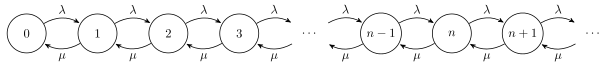
\includegraphics[scale=0.35]{MM1-queue.png}
\end{figure}

\subsection{M/M/c}
\begin{flalign*}
    & \rho = \frac{\lambda}{c\mu} 
    & c\mu > \lambda \text{  [Stability condition]} \\
    & \pi_0 =  (\frac{\lambda}{\mu})^c \frac{1}{1 - \rho} 
    % TODO Fix from notes:
    & \pi_i = 
        \begin{cases}
            \frac{\lambda^i}{i!\mu^i} \pi_0,  & \text{if } i < c \\
            \frac{\lambda^i}{c!\mu^ic^{i-c}} \pi_0,              & \text{if } i \geq c 
        \end{cases}&  \\ 
    & \mathbb{E}[N] = \lambda \mathbb{E}[R] 
    & \mathbb{E}[N_Q] = \lambda \mathbb{E}[R_Q] \\
    & \mathbb{E}[R] = \mathbb{E}[R_Q] + \mathbb{E}[S] = \mathbb{E}[R_Q] +  \frac{1}{\mu} \\
    & \mathbb{E}[R_Q] = \frac{(\frac{\lambda}{\mu})^c \mu}{(c-1)! (c\mu - \lambda)^2} \\
    & P(\text{job is queued}) = \sum_{i=0}^\infty \pi = \frac{1}{c!}(\frac{\lambda}{\mu})^c \frac{1}{1-\rho} \pi_0
    & \text{[Erlang C Formula]}
\end{flalign*}

\begin{figure}[H]
    \vspace{-0.25cm}
    \centering
    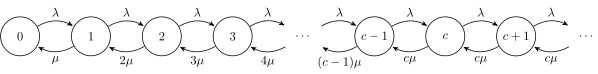
\includegraphics[scale=0.35]{MMC-queue.png}
\end{figure}

\vspace{-0.25cm}
\subsection{M/M/$\infty$}
\begin{flalign*}
    & \rho = \lambda/\mu 
    & \mu > \lambda \text{ [Always Stable]}\\
    & \pi_0 =  e^{-\frac{\lambda}{\mu}} = e^{-\rho}
    & \pi_i = \frac{(\lambda/\mu)^i}{i!} e^{-\frac{\lambda}{\mu}} = \frac{\rho^i}{i!} e^{-\rho} \\
    & \mathbb{E}[N] = \frac{\lambda}{\mu} = \rho 
    & \mathbb{E}[N_Q] = 0 \\
    & \mathbb{E}[R] = \frac{1}{\mu} = \mathbb{E}[S] 
    & \mathbb{E}[R_Q] =  0 \\
\end{flalign*}

\begin{figure}[H]
    \vspace{-1cm}
    \centering
    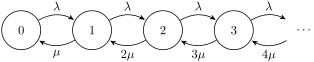
\includegraphics[scale=0.4]{MMinfinity-queue.png}
\end{figure}


\subsection{Birth-Death Process}
CTMC where state transitions increase or decrease by a constant factor.
%TODO check notes for pi_0
\[
    \pi_0 = \frac{1}{1 + \sum_{k=1}^{\infty} \prod_{i=1}^k \frac {\lambda _{i-1}}{\mu_i} }
\]
\[
    \pi_i = \frac{\prod_{j=0}^{i-1} \lambda_j}{ \prod_{j=1}^{i} \mu_j}\pi_0
\]

\subsection{Threshold System}
$T>0$, Arrival rate $s$, processing rate $s$. If $r > s, N \to 0$. If $s >r, N \to \infty$.  
\[
    \pi_0 = \frac{1}{1 - \frac{r}{s}} (\frac{s}{r})^T-1
\]
\[
    \pi_i = 
        \begin{cases}
            (\frac{s}{r})^i \pi_0,  & \text{if } i < T \\
            (\frac{s}{r})^{i-T} (\frac{r}{s})^2 \pi_0, & \text{if } i \geq T
        \end{cases}
\]

\subsection{Jackson Networks}
\begin{enumerate}
    \item 
    External arrivals form a Poisson process
    \item
    All service times are exponentially distributed and the service discipline at all queues is first-come, first-served
    \item
    internal routing of jobs between servers is probabilistic
    \item
    The utilization of all of the queues is less than one
\end{enumerate}
Solved via markov model

\begin{enumerate}
    \item \textbf{Markov Chain:} We may solve the corresponding Discrete Time Markov Chain to find its steady state distribution, $\mathbb{E}[N]$, and $\mathbb{E}[R]$. If there are $N$ jobs and $k$ nodes, we will have a lower bound of $\Omega(\binom{N+k-1}{k-1}^2)$ when solving the system of equations.
    \item \textbf{Product form:} Using a temporary value for each node's arrival rate, $\bar \lambda$, determine the ratios between the balance equations and then recover the real values using the actual arrival rate, $\lambda$, finding the steady-state distribution, $\mathbb{E}[N]$, and $\mathbb{E}[R]$. Still suffers from a combinatorial explosion in complexity with a lower bound of $\Omega(\binom{N+k-1}{k-1})$.
    \item \textbf{Mean Value Analysis:} Uses the Arrival Theorem in a recursive algorithm to analyse specific nodes when there are $N$ jobs in the system. We only have access to expectations and utilization of specific nodes, i.e. $\mathbb{E}[R_i]$, $\mathbb{E}[N_i]$, $\rho_i$ but is more performant with an upper bound of $\mathcal{O}(Nk)$. 
\end{enumerate}

\subsection{M/G/1}

\begin{itemize}
    \item Markovian (modulated by a Poisson process), service times have a General distribution and there is a single server
    \item $\mathbb{E}[S] = \frac{1}{\mu}$
    \item high variance in service distribution $\implies$ high response time
    \item Has equal $\mathbb{E}[N]$ for all blind non-pre-emptive service policies
\end{itemize}

\subsection{Pollaczek–Khinchine formula}
\[
 \mathbb{E}[N] = \rho + \frac{\rho^2 + \lambda^2 \sigma_s^2}{2(1-\rho)}
\]

\section{Service Policies}
Blind and non-blind policy relates to knowledge of job size on arrival. If service times that jobs require are known, then the optimal scheduling policy is shortest remaining processing time (SRPT).
\begin{itemize}
    \item first-come, first-served (FCFS) 
    \item processor sharing (PS) where all jobs in the queue share the service capacity between them equally
    \item last-come, first served (LCFS) with/without preemption where a job in service may or may not be interrupted with work being conserved
    \item  generalized foreground-background (FB) scheduling also known as least-attained-service where the jobs which have received least processing time so far are served first and jobs which have received equal service time share service capacity using processor sharing
    \item shortest job first (SJF) with/without preemption, where the job with the smallest size receives service
    \item shortest remaining processing time (SRPT) where the next job to serve is that with the smallest remaining processing requirement
\end{itemize}

\section{Failure/Hazard Rate}
\begin{itemize}
    \item Increasing Failure Rate (IFR): h(t) is non-decreasing in t, the expected remaining work is decreasing, non pre-emptive is preferable.
    \item Decreasing Failure Rate (DFR): h(t) is non-increasing in t, the expected remaining work is increasing, pre-emptive policy is preferable.
\end{itemize}
\begin{flalign*}
    & \quad \quad h(t) = \frac{f(t)}{1 - F(t)}
    & \mathbb{E}[\text{Remaining time}] = \frac{1}{h(t)} \qquad \\
    & \quad \quad X \sim uniform(a,b) \text{ (IFR)} \implies
    & h(t) = \frac{1}{b-t} \qquad \\
    & \quad \quad X \sim exp(\lambda) \text{ (IFR and DFR)} \implies
    & h(t) = \frac{\lambda e^{-\lambda t}}{1-(1-e^{-\lambda t})} \qquad
\end{flalign*}
\[
\text{Time average Excess} = \mathbb{E}[S_c] = \frac{\mathbb{E}[S_c]}{2\mathbb{E}[S]}
\]
\[
    \mathbb{E}[R_Q] = \frac{\rho}{1-\rho} \mathbb{E}[S_c]
\]

\section{Pareto Distribution}
\begin{itemize}
    \item popular DFR, "80-20 rule", pre-emptive policy is preferable
    \item 50\% of the load on the system comes from 1\% of the jobs
    \item $\alpha$ shape parameter, $\alpha =1, X > t \implies P(X>2t) = \frac{1}{2}$
    \item $ 0 < alpha < 1$, $Var(X) = \infty$, $\mathbb{E}[X] = \infty$
    \item Survival Function:
\end{itemize}
\[
{\displaystyle {\overline {F}}(x)=\Pr(X>x)={\begin{cases}\left({\frac {x_{\mathrm {m} }}{x}}\right)^{\alpha }&x\geq x_{\mathrm {m} },\\1&x<x_{\mathrm {m} },\end{cases}}}
\]
\section{Misc}
\begin{itemize}
    \item 
     $\sum_{i=0}^\infty \alpha^i = \frac{1}{1-\alpha}, |\alpha| < 1 $.
    
    \item
    $h = \frac{f}{g} \implies h' = \frac{f'g -fg'}{g^2}$
    
    
    \item
    Max system utilization $\implies$ only bottleneck utilization is 100\%
    
    \item
    Want to minimize $\mathbb{E}[R]$ and maximize $X$.
    
    \item
    Operation Laws work regardless of distributions of random variables

    \item
    exponential distributions are a very good assumption for modeling arrivals, but only moderately good for modelling processing times
\end{itemize}

\end{multicols*}

\end{document}
